\section{Data engineering: from EDGAR to a point-in-time store}
\label{sec:data}

\subsection{Ingestion and storage}

Two ingestion paths run in parallel by design. The SEC DERA
structured datasets ($\sim$53 quarterly archives) are cheap and carry
the other-manager graph, but begin in 2013Q2 and inherit the SEC's
own parsing unaudited. The raw-filing path (SGML envelopes; XML after
2013, fixed-width layouts before) covers the whole archive and is
auditable, at one HTTP request per filing. A cross-validation routine
re-parses a random sample of raw filings and compares row counts and
value totals against DERA; neither source can check itself, and
agreement below 95\% halts the pipeline. The sample begins in 2013Q2
where the two paths overlap and the structured OTHERMANAGER graph is
available --- earlier eras are parseable but single-sourced, and we
prefer a shorter sample with a second witness.

Every holding row carries two dates: the period it describes and the
timestamp at which it became public (EDGAR acceptance). The store's
only read path for research, \texttt{as\_of(period, knowledge\_date)},
materializes both the current and prior quarter at the same knowledge
date, so a quarter-over-quarter change never mixes what was known
then with what is known now. Three mechanical look-ahead channels are
closed at this layer: late filings (a filer's book enters the panel
only after its acceptance timestamp), amendments (a correction
filed in March cannot retroactively improve a January decision), and
restatement semantics.

\subsection{Amendments, value scale, identity}

Amendment handling follows the cover page, never a heuristic:
\texttt{RESTATEMENT} replaces the filer's table for the period;
\texttt{NEW HOLDINGS} is additive (typically a lapsed
confidential-treatment order); a missing declaration is treated as a
restatement, the conservative choice. Misreading an additive
amendment as a restatement silently deletes a quarter's book ---
this failure mode is pinned by a test. An amendment is a
\emph{version} of its original, and never competes with it in any
largest-book logic. Value scale (the 2022--2023 thousands-to-dollars
cutover) is detected per filing keyed on the \emph{filing} date, with
loud outlier flags for the tail of filers that ignores the rule.
Filer identity is resolved by union-find over explicit evidence
(shared filings, CIK succession); name-similarity methods only
propose, and any merge requires a manual entry in a reviewed
configuration file --- nothing in the pipeline merges on string
distance alone.

\subsection{When information actually arrives}
\label{sec:delays}

The decision clock used throughout is quarter-end $+45$ calendar
days, the statutory deadline. Table~\ref{tab:delays} and
Figure~\ref{fig:delays} justify it with the acceptance-timestamp
distribution over 254{,}630 original filings: the median filer
reports 41 days after quarter end, half of all filings arrive in the
final five days before the deadline, 89.4\% have arrived by D+45 and
98.1\% by D+60; the 99th percentile is 128 days and the maximum
observed 400. Lateness is sticky (a filer late once is late again
41\% of the time), so late books are a persistent subpopulation, not
noise. A per-name ragged-entry design --- entering each stock on the
day its holder's filing actually arrived --- adds $+0.2\%$/yr
($t\approx 0$) over the batch clock (Section~\ref{sec:tactical}): the
information is so concentrated at the deadline that waiting for it
costs nothing.

\begin{table}[t]
\centering\small
\caption{Filing-delay distribution, original 13F filings 2013--2026
($n=254{,}630$). The D+45 batch clock is justified by measurement:
89\% of books are public by the statutory deadline and the ragged
per-name alternative adds nothing (Section~\ref{sec:tactical}).}
\label{tab:delays}
\begin{tabular}{lrrrrrrr}
\toprule
 & median & p90 & p99 & max & $\le$D+40 & $\le$D+45 & $\le$D+60 \\
\midrule
delay (days) & 41 & 46 & 128 & 400 & 49.9\% & 89.4\% & 98.1\% \\
\bottomrule
\end{tabular}
\end{table}

\begin{figure}[t]
\centering
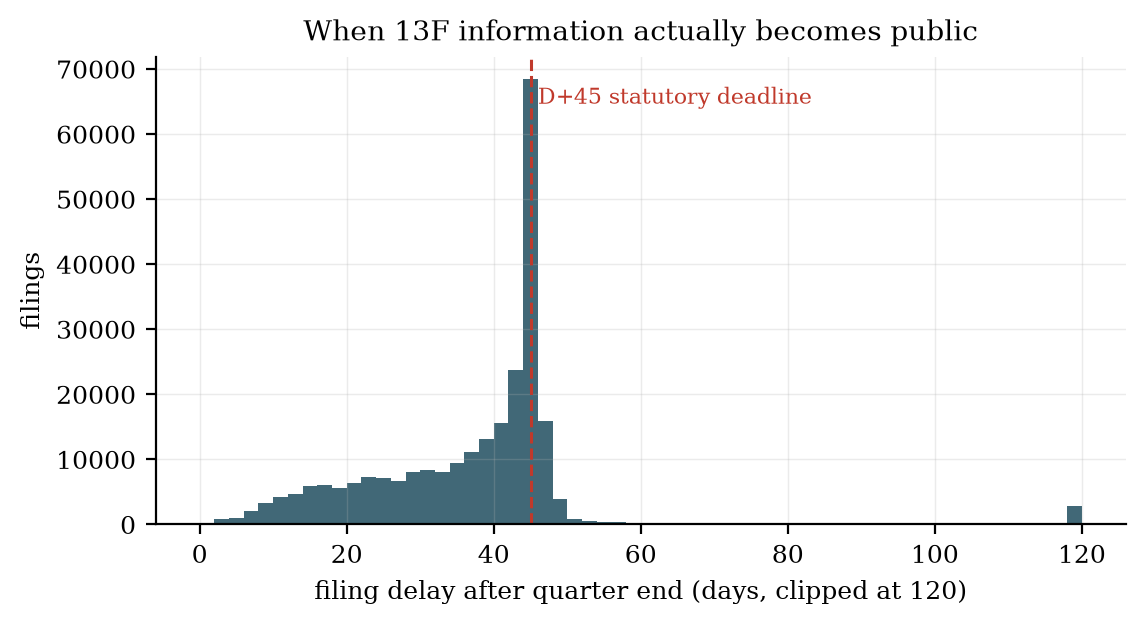
\includegraphics[width=.72\linewidth]{figs/f9_delays.png}
\caption{Acceptance-timestamp distribution. Half of all filings land
in the last five days before the statutory deadline (dashed line).}
\label{fig:delays}
\end{figure}

\subsection{The crosswalk, and the audit that mattered}
\label{sec:crosswalk}

Holdings identify securities by CUSIP; the price panel is keyed by
ticker. The map is CUSIP $\to$ issuer name (from the filings
themselves) $\to$ \emph{current} ticker by normalized-name match
against the exchange directory, ambiguous names discarded, with
manual resolution of edge cases (human in the loop). Three failure
modes were analyzed separately. Ticker renames (\texttt{FB}$\to$%
\texttt{META}) are correct by construction, because the vendor
reindexes history under the current symbol. Ticker recycling fails
\emph{closed}: history of a delisted issuer is never spliced under a
recycled symbol, so affected periods drop out at the price floor ---
exclusion, never mispricing (4.5\% of tickers flagged; inspected
cases are known spin-offs and IPOs). CUSIP reassignment by the same
issuer --- the genuine blind spot --- was measured directly: 1{,}574
events over 51 quarters, contaminating 0.22\% of position-exit flow;
exit-based signals are safe uncorrected.

Late in the project a value-weighted audit --- prompted by the simple
question ``what happens when tickers change?'' --- found that
\textbf{46.4\% of 2025Q4 book value was unmapped}. The cause was not
renames but EDGAR's name abbreviations (``LILLY ELI \& CO'',
``INTERNATIONAL BUSINESS MACHS''), which defeat exact matching
precisely on the mega-caps every value book holds. Count-weighted
coverage had looked healthy throughout; the lesson we record is that
\emph{coverage audits must be value-weighted}. The fix: the top 250
unmapped CUSIPs by value (65\% of the hole) hand-mapped and verified
individually; 61 new price histories fetched; caches stitched;
non-ETF value coverage raised from 63\% to 85.4\%, with a documented
ladder to $\sim$93\% (identifier-service tail) and $\sim$98\%
(CRSP-tier, delistings).

\subsection{The re-verification campaign and one retraction}
\label{sec:campaign}

Because coverage selection could in principle manufacture or hide
results, every material verdict was re-run on the expanded universe:
24 re-runs. The pre-registered expectation was that the hole was
quasi-random with respect to signals (EDGAR name formatting does not
predict returns), so levels could move where mega-caps matter but
verdicts should stand. Twenty-one verdicts were unchanged; two
instruments \emph{strengthened} with completer books (the flow
instrument's selling contrast from $t=+13.8$ to $t=+20.9$; synthetic
short interest's correlation with actual short interest from $0.47$
to $0.55$); NCB replicated inside its historical band and survived
two random 50\%-coverage halvings ($t=+3.45/+2.79$), the generic
proof that quasi-random coverage cannot flip verdicts.

One result flipped and is retracted: a daily overlay claiming that a
synthetically detected ``stressed'' manager's top holdings
underperform over the following five days ($t=-2.16$ on the old
universe) went to $t=+0.37$ on complete books and is dead even inside
its own sub-window. The diagnosis is an eligibility-selection
artifact: coverage filters had excluded managers holding unmapped
mega-caps, biasing the manager sample toward a stratum where the
effect appeared. The research funnel had already declined to promote
the result (net returns too thin); the audit converted ``not
promotable'' into ``false.'' We keep both the machinery (reused by
the risk monitors of Section~\ref{sec:tactical}) and the negative
finding.
